\subsection{WP0 Management}

{\bf Work package manager: R.\,Preece.}

The DUNE-UK production project is fully integrated into the larger LBNF/DUNE-UK project the structure, which is presented in Figure \ref{fig:organogram}. 
\begin{figure}[htb]
    \centering
    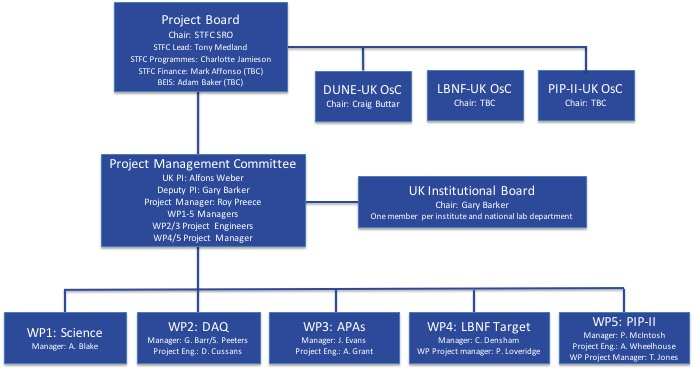
\includegraphics[width=0.9\textwidth]{figs/organogram.jpg}
    \caption{Organogram of the UK LBNF/DUNE project}
    \label{fig:organogram}
\end{figure}

The overall project will be managed by the project management committee (PMC), which consists of the overall PI (Weber), the overall PM (Preece), all the work package mangers, WP project managers and engineers. Additionally the deputy-PI (Barker), will take a leading role in the DUNE part of the project (WP1-3). The role of the PMC, which is chaired by the project PI, is to track the progress of the overall project and to facilitate the reporting to STFC, the different Oversight Committees and Project Board. It will meet monthly to discuss progress and any issues, with the aim of ensuring effective communication within the UK project. 

DUNE-UK consists of sixteen institutes (universities and national lab departments), which are each represented in the  LBNF/DUNE-UK Institute Board (IB). The LBNF/DUNE-UK IB will ratify the overall project management (PI, PM, WP-managers/engineers), the resource allocation to the different institutions and the documentation to be submitted to the PB and the OsCs.

The Working Margin (WM) is managed across the overall project (WP1-5). Allocation of these resources will be agreed by the PMC, with the overall Project Manager taking responsibility for tracking the overall progress of the project and monitoring cost and schedule. 

The following sections relate to WP1-3 of the LBNF/DUNE project, which form part of this proposal. The corresponding resources are held centrally by WP0.

\subsubsection{Travel}
The cost of travel has been estimated, bottom-up, for the different work-packages. In addition overall travel to collaboration meetings and workshops and for reviews and management have been taken into account. The summary can be found in table \ref{tab:travel}. Travel fund will be managed overall by the DUNE project and will be held at STFC/RAL/PPD. 
\begin{table}[htb]
    \centering
    \begin{tabular}{|c||c|c|c|c|c|c|c|c||r|}
        \cline{2-10} \multicolumn{1}{c|}{\ } & \multicolumn{9}{c|}{cost in k£}\\
         \cline{2-10}
         \multicolumn{1}{c|}{\ } & 19/20 & 20/21 & 21/22 & 22/23 & 23/24 & 24/25 & 25/26 & 26/27 & total\\
         \cline{2-10}\hline
         \multicolumn{10}{|c|}{General/WP0 }\\
         \hline
         collab. mtg.    &  90 & 180 & 180 & 180 & 180 & 180 & 180 &  90 & 1,260 \\
         UK mtg.         &  13 & 25  &  25 &  25 &  25 &  25 &  25 & 13  & 175   \\
         management mtg. &   9 & 18  &  18 &  18 &  18 &  18 &  18 &   9 & 126  \\
         LTA             &     &     &     &     &     &  40 &  40 &  20 & 100  \\
         \hline
         \hline
         \multicolumn{10}{|c|}{WP1 }\\
         \hline
         int.\,WS       & 8 & 15  & 15  &  15 & 15  & 15  & 15 & 8 & 105  \\
         nat.\,WS       & 3 & 6   & 6   & 6   & 6   & 6   &  6 & 3 & 42 \\
         \hline\hline
         \multicolumn{10}{|c|}{WP2 }\\
         \cline{1-10}
         int.\,WS      &  9  & 18  & 18  & 18  & 18  &     &    &    & 81  \\
         nat.\,WS      &   3 & 6   &  6  & 6   &   6 &     &    &    & 27  \\
         installation  &     & 60  & 120 & 120 & 60  &     &    &    & 360  \\
         LTA           &     &     & 20  & 20  & 20  &  20 & 20 & 10 & 110  \\
         \hline\hline
         \multicolumn{10}{|c|}{WP3 }\\
         \cline{1-10}
         int.\,WS      &  15 & 30  & 30  & 30  & 30  & 30  &    & & 165  \\
         nat.\,WS      &   3 &  6  &  6  & 6   &  6  &  6  &    & & 33  \\
         installation  &     & 60  & 60  & 60  & 60  &  60 &    & & 300  \\
         LTA           &     & 10  & 20  & 20  & 20  &  20 &    & & 90  \\
         \hline\hline
         total           & 152 & 374 & 464 & 584 & 584 & 540 & 304 & 152 & 3,154\\
         \hline
    \end{tabular}
    \caption{Breakdown of travel request by activity. \color{red} some fantasy, needs to be fixed.}
    \label{tab:travel}
\end{table}
We have made the following assumption.
\begin{itemize}
    \item The cost for an international WS or collaboration meeting is k£ 1.5 per traveller. Collaboration meetings are attended by 50 UK people, while WS are typically attended by 5.
    We assume that there will be 5 collaboration meetings per year and a total of 5 international WSs.
    \item We will hold two 2-day UK meetings each year attended by 80 collaborators at a cost of £ 250 per trip.
    \item
    LTA cost at SURF (USA) is k£ 20/year. We expect to have several people at SURF during installation, one for the DAQ one for APA
    \item {\color{red} This needs to be fleshed out!}
\end{itemize}

\subsubsection{Common Fund}
The common fund contributions will be held in WP0, details of the expected contributions can be found in section \ref{sec:CF}

\subsubsection{Working Allowance}

{\color{red}this is a section for Roy}

\begin{itemize}
    \item has been calculated and profiled according to risk.
    \item WA is held across overall LBNF/DUNE project
    \item spending limits and process
    \item use of WA to increase scope?
\end{itemize}

